
\chapter{Introduction}

\section{Problem Statement}

In the era of social media, Fake news or fabricated content is exponentially growing. Social media platforms are set up to push the most viewed content, and controversial topics get way more interactions.
Facebook shows an endless stream of items from all over the web. 
Click an interesting headline and you may end up on a Fake news site. 
Fake stories have no reputation to maintain and no incentive to stay honest; Social media becomes a breeding ground for Fake news, As a result of spreading fake news the public opinion could be biased and manipulated for instance in the 2016 US presidential election and how spreading Fake news influenced the presidential election and favored a specific candidate. \\
This raises our aim to implement an application that could mitigate Fake news by incenting users to share and verify stories and build a reputation system for the story creators and considering the user's location or how close or far away from an event in our equation.
By taking into account both the users' reputation score and the location´s trustworthiness we will ensure that the users will report only the accurate stories. 

	\section{Introductory Walk-Through}
The spread of social media and integrating it as an essential part of our daily life has a tremendous effect on spreading fake news. Many adults prefer getting news from the social media platforms like Facebook and Twitter more than the legacy ways like newspaper and broadcast, with the advance of technology it becomes trivial to manipulate images and videos.   
    Our mission is to mitigate fake news with our platform we incent users to publish and rank nearby events based on their reputation. By using hyperledger technology it will be hard to manipulate the data once it's stored on the blockchain.\\ 

We are using a ranking scheme to increase the trustworthiness of the users, Also the user's location is taken into consideration when calculating the ranking score. We gave more weight to the users, which their location is closer to the event they are judging. 
By virtue of the chain code or smart contract, which will be responsible for handling the business logic and rank the events based on users location and trustworthiness. The architecture of our application could be described in particular as below:      


       \begin{enumerate}
	 \item {A user can capture an event or text and upload it using our android application to the blockchain.}
	 \item {The event's data will be stored permanently on the blockchain and it will be impossible to be altered.} 
	 \item {Our application will fetch and display the events to the nearby users.} 
         \item {The users in the close-by area will be able to judge the events and upload comments and further media files that approve or disapprove the events.  we are restricting the participation of the users in judging events, and only legitimate users that their locations are in the nearby area will be eligible to vote. \footnote[1]{collecting time and location evidence in order to assure that the users were in the nearby area and their location wasn't spoofed  is part of a separate bachelor thesis running in parallel.} }
         \item {Depending on the other users reviews on the assessed event, the chaincode will update the trustworthiness value of the event \footnote[2]{Ranking the trustworthiness of the events and the users will be based on the reviews of the event in addition to the trusted code execution is part of a separate thesis running in parallel. } }
          \item {The chaincode will update the event creator's reputation score based on the reviews that his events received. In other words, An event which received good reviews will get a more trustworthiness score also it will increase the event creator's reputation score and gives him more credits on our platform.} 
	\end{enumerate}

\noindent In \hyperref[fig:appflow]{Figure 1.1} we describe the previously mentioned procedures as an overview of our platform.
	\begin{figure}[H]
	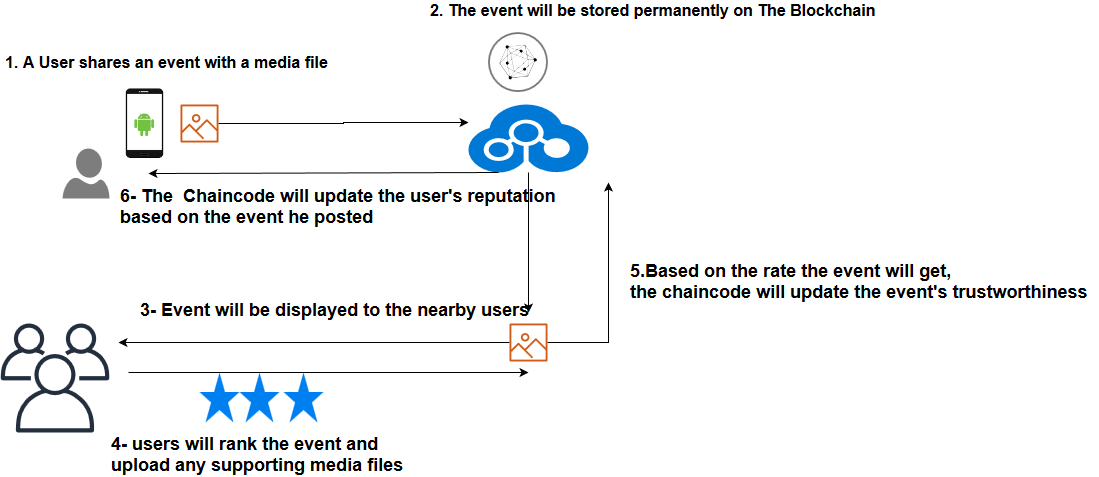
\includegraphics[width=15cm,height=12cm]{images/appflow.png}
	\caption{The Application Walkthrough}
	\label{fig:appflow}
	\end{figure}

\cleardoublepage

\section{Architecture}
The platform would be dismantled into three main components: 
\begin{itemize}
  \item The Hyperledger fabric network.
  \item The Backend and Fabric SDK. 
  \item The Android Development. 
\end{itemize}


\noindent In order to fully grasp the whole components of the platform. In chapter 2 we will start with the necessary background information about the Blockchain, The terminologies, And the main components of Hyperledger fabric for example peers, chaincode, transactions .etc. \\
In chapter 3, We will discuss the backend, API Design and how the API requests will be consumed and the way that Node.js SDK handles the requests, also how the SDK interacts with hyperledger fabric network and the chaincode. \\
Finally, We will discuss the Android application design, UI elements, The Main activities and classes in depth with all the implemented functionality. \hyperref[fig:architecture]{Figure 1.2} depicts all the architecture overview of the platform. 
\begin{figure}[H]
	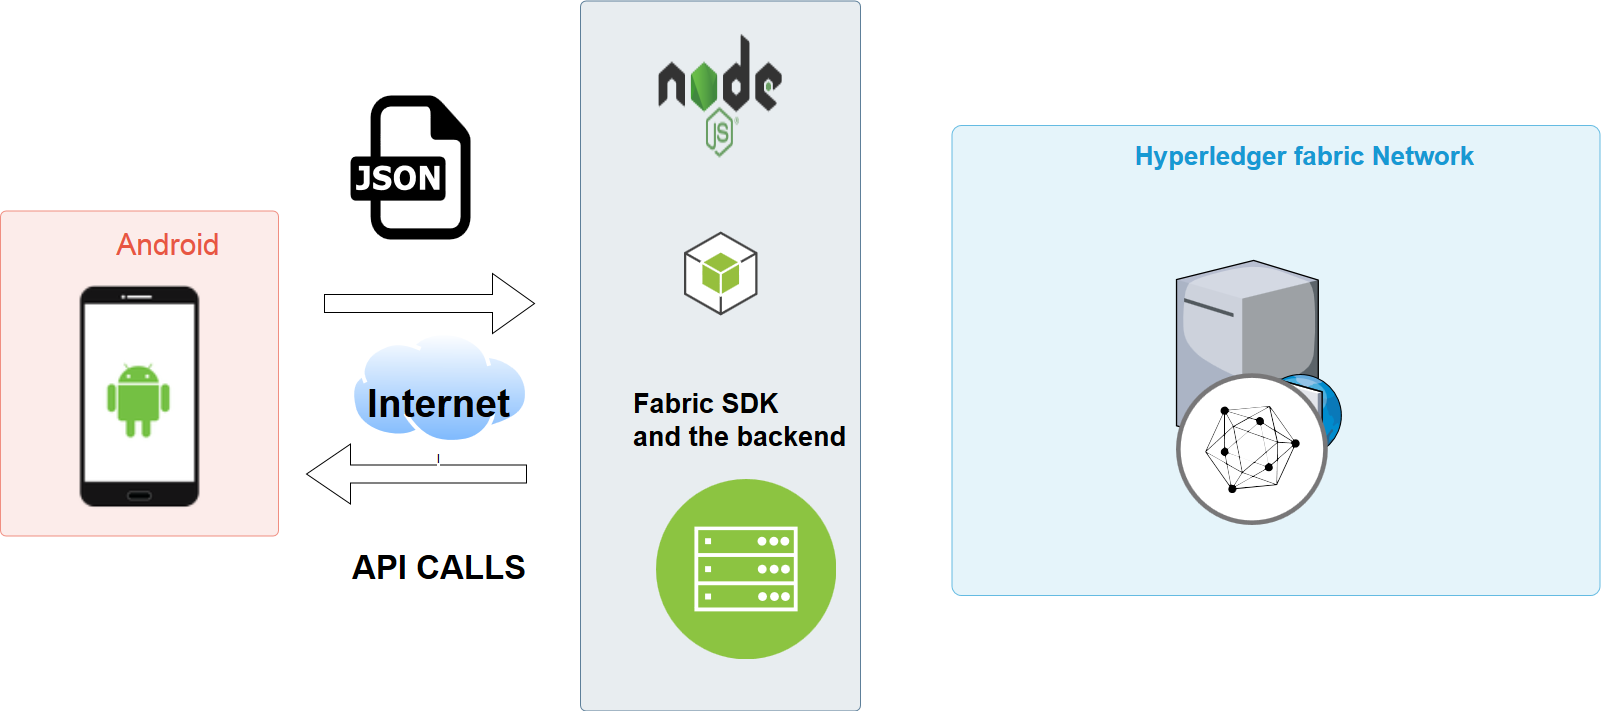
\includegraphics[width=15cm,height=10cm]{images/architecture.png}
	\caption{Architecture Overview}
	\label{fig:architecture}
	\end{figure}

      

 


      